\documentclass[spanish]{beamer}
\usepackage[ansinew]{inputenc} % Acepta caracteres en castellano
\usepackage[spanish]{babel}    % silabea palabras castellanas
\usepackage{amsmath}
\usepackage{mathtools,cancel} % cancela con una flecha \cancelto{0}{XXXX}
\renewcommand{\CancelColor}{\color{red}} %change cancel color to red
\usepackage{amsfonts}
\usepackage{amssymb}
\usepackage{dsfont}
\usepackage{graphicx}
\usepackage{geometry}
\usetheme{Madrid}
\usecolortheme{beaver}
\usepackage{textpos}
% Logo  en el comienzo 
\addtobeamertemplate{frametitle}{}{%
\begin{textblock*}{100mm}(.85\textwidth,-1cm)
{\includegraphics[height=0.4in, keepaspectratio=true]{/Users/luisnunez/Dropbox/MisDocumentos/UIS/UISImagenInstitucional/UISLOGO.png}}
\end{textblock*}}

\begin{document}

\title{\textbf{�rbitas y fuerzas centrales} }
\author[L.A. N��ez]{\textbf{Luis A. N��ez}}  
\institute[UIS]{\textit{Escuela de F�sica, Facultad de Ciencias, } \\
\textit{Universidad Industrial de Santander, Santander, Colombia } \\
{\includegraphics[height=0.4in, keepaspectratio=true]{/Users/luisnunez/Dropbox/MisDocumentos/UIS/UISImagenInstitucional/UISLOGO.png}}
}
\date{\today}
\maketitle


\begin{frame}
\frametitle{Agenda}
  \tableofcontents
\end{frame}


%%%%% Diapo 1
\section{Problema de dos cuerpos}
\frame{
  \frametitle{Problema de dos cuerpos}
   \begin{itemize}  
  	\item<1-> Consideremos dos part�culas $m_1$ y $m_2$ en $\mathbf{r}_1$ y $\mathbf{r}_2$, respecto a un origen $O$ de un sistema de referencia inercial. 
	\item<2-> Supongamos que las part�culas interaccionan mediante un potencial que depende solamente de sus posiciones relativas, $V\left(\mathbf{r}_1, \mathbf{r}_2\right)=V\left(\mathbf{r}_2-\mathbf{r}_1\right) $. Se conoce como el problema de dos cuerpos. 
	\item<3-> Posee seis grados de libertad: tres coordenadas para $\mathbf{r}_1$ y  tres para $\mathbf{r}_2$.
	\item<4-> Definimos el vector de posici�n del centro de masa del sistema como $\mathbf{R}=\frac{m_1 \mathbf{r}_1+m_2 \mathbf{r}_2}{m_1+m_2}$ y posici�n relativa como $\mathbf{r}=\mathbf{r}_2-\mathbf{r}_1$
	\begin{figure}[t]
		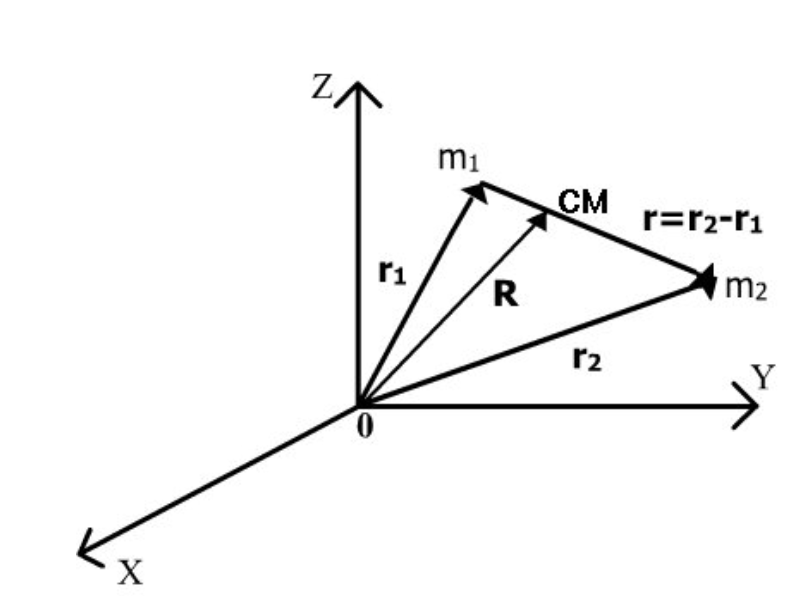
\includegraphics[width=2.0in]{Figuras/DosCuerpos.png}
   	\end{figure}
    \end{itemize}
}
%%%%% Diapo 2
\section{Los grados de libertad}
\frame{
  \frametitle{Los grados de libertad}
   \begin{itemize}  
  	\item<1-> Las posiciones de las part�culas relativas al centro de masa son $\mathbf{r}_1^{\prime}  =\mathbf{r}_1-\mathbf{R}$ y $\mathbf{r}_2^{\prime} =\mathbf{r}_2-\mathbf{R}$
	\item<2-> Es decir: $\mathbf{r}_1^{\prime}=\mathbf{r}_1-\frac{m_1 \mathbf{r}_1+m_2 \mathbf{r}_2}{m_1+m_2}=\frac{m_2\left(\mathbf{r}_1-\mathbf{r}_2\right)}{\left(m_1+m_2\right)}=-\frac{m_2}{\left(m_1+m_2\right)} \mathbf{r}$ y 
	$ \mathbf{r}_2^{\prime}=\mathbf{r}_2-\frac{m_1 \mathbf{r}_1+m_2 \mathbf{r}_2}{m_1+m_2}=\frac{m_1\left(\mathbf{r}_2-\mathbf{r}_1\right)}{\left(m_1+m_2\right)}=\frac{m_1}{\left(m_1+m_2\right)} \mathbf{r}$
	\item<3-> La energ�a cin�tica total del sistema ser� $T=T_{\mathrm{cm}}+T_{\mathrm{rel}}$
	\item<4-> Entonces $T_{\mathrm{cm}} =\frac{1}{2} M_T \dot{\mathbf{R}}^2=\frac{1}{2}\left(m_1+m_2\right) \dot{\mathbf{R}}^2$
	\item<5-> y $T_{\mathrm{rel}} =\frac{1}{2} m_1 \dot{\mathbf{r}}_1^{\prime 2}+\frac{1}{2} m_2 \dot{\mathbf{r}}_2^{\prime 2} =\frac{1}{2} \frac{m_1 m_2^2}{\left(m_1+m_2\right)^2} \dot{\mathbf{r}}^2+\frac{1}{2} \frac{m_1^2 m_2}{\left(m_1+m_2\right)^2} \dot{\mathbf{r}}^2 =\frac{1}{2} \frac{m_1 m_2}{\left(m_1+m_2\right)} \dot{\mathbf{r}}^2$
	\item<6-> y si definimos la masa reducida, $\mu \equiv \frac{m_1 m_2}{\left(m_1+m_2\right)}$
	\item<7-> El Lagrangiano del sistema es 
	$\mathcal{L}(\mathbf{r}, \mathbf{R}, \dot{\mathbf{r}}, \dot{\mathbf{R}}) =T-V\left(\mathbf{r}_2-\mathbf{r}_1\right) =\frac{1}{2}\left(m_1+m_2\right) \dot{\mathbf{R}}^2+\frac{1}{2} \mu \dot{\mathbf{r}}^2-V(\mathbf{r})$
	\item<8-> Los seis grados de libertad del sistema se describen mediante las componentes de los vectores $\mathbf{r}$ y $\mathbf{R}$.
    \end{itemize}
}

%%%%% Diapo 2
\section{La equivalencia unidimensional}
\frame{
  \frametitle{La equivalencia unidimensional}
   \begin{itemize}  
  	\item<1-> Las componentes cartesianas de $\mathbf{R}$ son coordenadas c�clicas, lo que implica $M_{\mathrm{T}} \dot{\mathbf{R}} \equiv (m_1+m_2)\dot{\mathbf{R}}=$ cte. \\ Es decir: {\bf el momento lineal total del sistema se conserva}
	\item<2-> Como no hay fuerzas externas sobre el sistema : $\mathbf{F}_{\text {externa total }}=0 \Rightarrow \mathbf{P}_{\mathrm{T}}=M_{\mathrm{T}} \dot{\mathbf{R}}=$ cte. El centro de masa se mantiene en reposo o se mueve con velocidad constante, $\dot{\mathbf{R}}=$ $\mathbf{v}_{\mathrm{cm}}=$ cte.
	\item<3-> Existir�n tres cantidades conservadas correspondientes a las tres componentes del momento lineal total o, equivalentemente, a las tres componentes de la velocidad del centro de masa.
	\item<4-> El t�rmino $T_{\mathrm{cm}}$, la energ�a cin�tica del centro de masa es constante y se omite en el Lagrangiano, $\mathcal{L}=\frac{1}{2} \mu \dot{\mathbf{r}}^2-V(\mathbf{r})$
	\item<5-> El problema de dos cuerpos se reduce al de una part�cula de masa $\mu$ en la posici�n relativa $\mathbf{r}(t)$ con respecto a un origen $O^{\prime}$.
	\begin{figure}[t]
		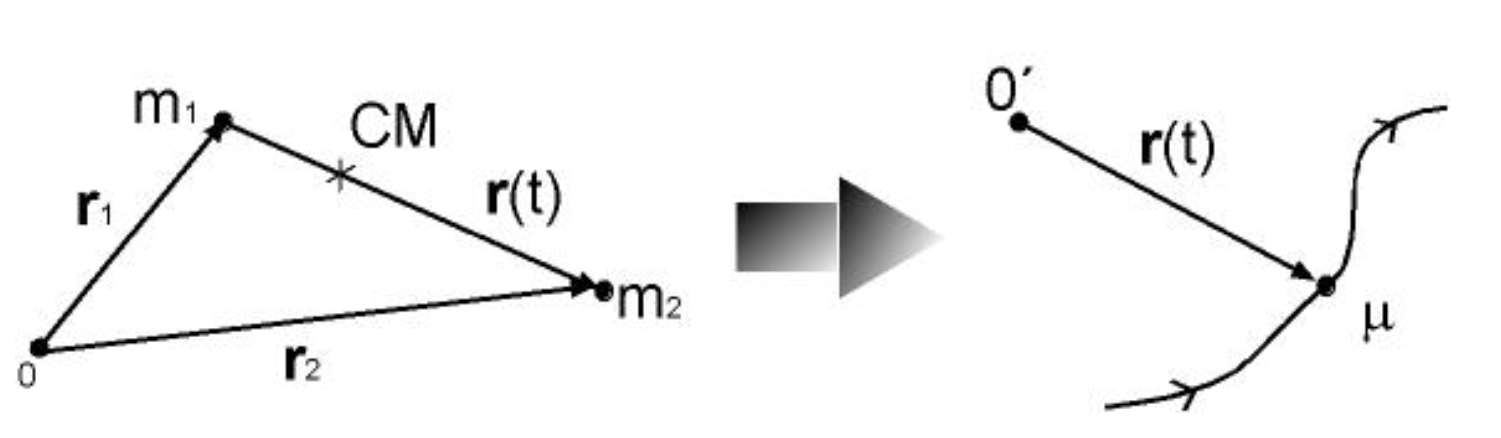
\includegraphics[width=1.7in]{Figuras/EquivalenciaDosCuerpos.png}
   	\end{figure}

    \end{itemize}
}

%%%%% Diapo 2
\section{Potenciales centrales, $V({\bf r})$}
\frame{
  \frametitle{Potenciales centrales, $V({\bf r})$}
   \begin{itemize}  
  	\item<1->  El problema se simplifica m�s para potenciales centrales, $V({\bf r})$.
	\item<2->   Entonces la fuerza central es $\mathbf{F}=-\nabla V({\bf r})=-\frac{\partial V}{\partial r} \hat{\mathbf{r}}=f({\bf r}) \hat{\mathbf{r}}$
	\item<3-> Las fuerza centrales no ejercen torque neto sobre las part�culas y el momento angular total ${\bf L}$ se conserva, $\boldsymbol{\tau} =\mathbf{r} \times f({\bf r}) \hat{\mathbf{r}}=0 \Rightarrow \boldsymbol{\tau} =\frac{{\rm d}  \mathbf{L}}{{\rm d} t}=0 \Rightarrow \mathbf{L}=\mathbf{r} \times \mathbf{p}=\text { cte }$
	\item<4-> La conservaci�n del vector momento angular total, ${\bf L}$, significa que tanto su direcci�n como magnitud son constantes.
	\item<5-> El movimiento de la part�cula de masa equivalente $\mu$ siempre ocurre sobre el plano ($\mathbf{r}, \mathbf{p})$ y se puede describir mediante dos coordenadas.
	\begin{figure}[t]
		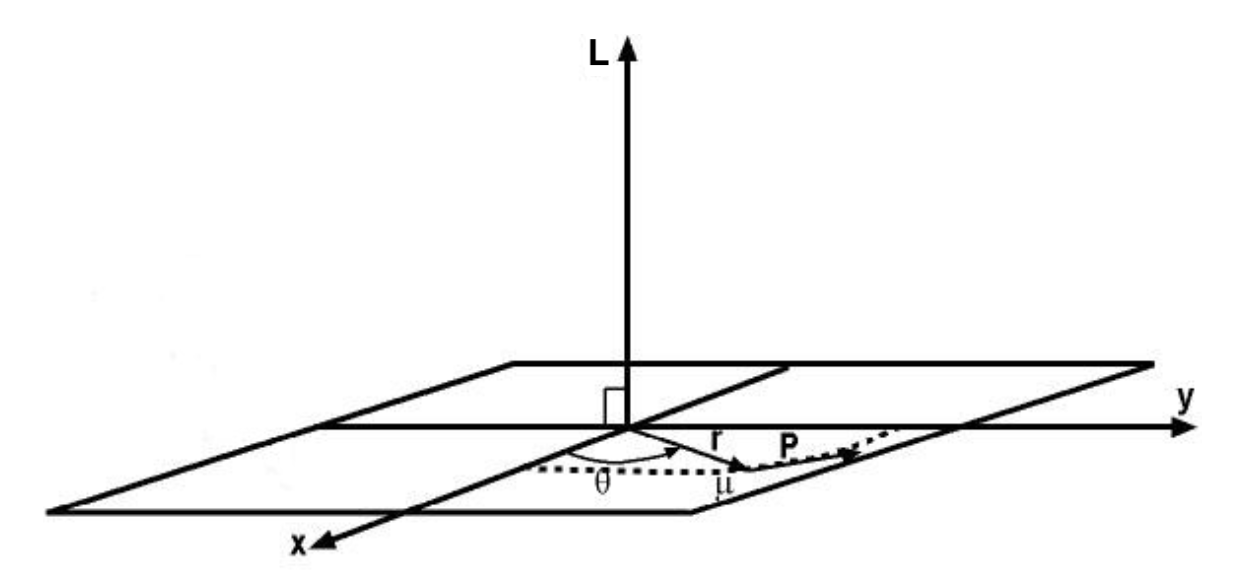
\includegraphics[width=1.9in]{Figuras/MomAngularConstante.png}
   	\end{figure}

    \end{itemize}
}
\section{Resolviendo en coordenadas polares}
\frame{
  \frametitle{Resolviendo en coordenadas polares}
   \begin{itemize}  
  	\item<1-> Las coordenadas polares generalizada $(r, \theta)$ implican \\
	$x=r \cos \theta \Rightarrow \dot{x}=\dot{r} \cos \theta-r \dot{\theta} \sin \theta \, ,$\\ $ y=r \sin \theta \Rightarrow  \dot{y}=\dot{r} \sin \theta+r \dot{\theta} \cos \theta$
	\item<2-> Luego, $\dot{\mathbf{r}}^2=v^2=\left(\dot{x}^2+\dot{y}^2\right)=\left(\dot{r}^2+r^2 \dot{\theta}^2\right)$
	\item<3-> El Lagrangiano ser�  $\mathcal{L}=\frac{1}{2} \mu\left(\dot{r}^2+r^2 \dot{\theta^2}\right)-V(r)$
	\item<4-> La coordenada $\theta$ es c�clica, entonces 
	$\frac{{\rm d} }{{\rm d} t}\left(\frac{\partial \mathcal{L}}{\partial \dot{\theta}}\right)-\frac{\partial \mathcal{L}}{\partial \theta}=0 \; \Rightarrow \frac{\partial \mathcal{L}}{\partial \dot{\theta}}=\mu r^2 \dot{\theta}=$  cte.
	\item<5-> La cantidad conservada es el momento conjugado a la coordenada angular $\theta$, i.e. $L=\mu r^2 \dot{\theta}=$ cte.
	\item<6-> El Lagrangiano es independiente del tiempo y el potencial es independiente de las velocidades, por lo que la energ�a mec�nica total se conserva, $E=\frac{1}{2} \mu \dot{\mathbf{r}}^2+V(r)=\frac{1}{2} \mu\left(\dot{r}^2+r^2 \dot{\theta}^2\right)+V(r)=$cte.
    \end{itemize}
}
%%%%% Diapo 2
\section{El Sistema es integrable}
\frame{
  \frametitle{El Sistema es integrable}
   \begin{itemize}  
  	\item<1-> Entonces, en el problema de dos cuerpos existen seis grados de libertad y al menos seis cantidades conservadas. Por lo tanto, se trata de un sistema integrable.
	\item<2-> Las seis cantidades conservadas $I_k\left(\mathbf{r}_1, \mathbf{r}_2, \dot{\mathbf{r}}_1, \dot{\mathbf{r}}_2\right)=C_k(k=1, \ldots, 6)$  del problema de dos cuerpos sujetos a un potencial central $V\left(\left|\mathbf{r}_2-\mathbf{r}_1\right|\right)=V(r)$ son:
	\begin{enumerate}
	\item Las tres componentes del vector velocidad del centro de masa $\dot{\mathbf{R}}$: $I_1=\dot{x}_{c m}=$ cte, $I_2=\dot{y}_{c m}=$ cte, $I_3=\dot{y}_{c m}=$ cte. Esto reduce el problema al movimiento del vector de posici�n relativa $\mathbf{r}$.
	\item La direcci�n del momento angular ${\bf L}=$ cte, reduce el movimiento a un plano y se expresa como $I_4=z=0$.
	\item La magnitud del momento angular $I_5=\mu r^2 \dot{\theta}=L$.
	\item La energ�a total $I_6=\frac{1}{2} \mu\left(\dot{r}^2+r^2 \dot{\theta}^2\right)+V(r)=E$.
	\end{enumerate}
	\item<3-> Las cantidades conservadas $E$ y $L$, permiten reducir el problema de dos cuerpos a un problema unidimensional equivalente y la integraci�n de las coordenadas $r$ y $\theta$, i.e. $E=\frac{1}{2} \mu \dot{r}^2+\frac{1}{2} \frac{L^2}{\mu r^2}+V(r)=$cte. 
    \end{itemize}
}
%%%%% Diapo 2
\section{Integrando el sistema}
\frame{
  \frametitle{Integrando el sistema}
   \begin{itemize}  
  	\item<1-> De la energ�a obtenemos $\dot{r}=\frac{{\rm d} r}{{\rm d} t}=\sqrt{\frac{2}{\mu}\left(E-V(r)-\frac{L^2}{2 \mu r^2}\right)}$
	\item<2-> Para $t=0$ y $r=r_0$ tenemos: 
	$t(r)=\sqrt{\frac{\mu}{2}} \int_{r_0}^r \frac{{\rm d}  r^{\prime}}{\sqrt{E-V\left(r^{\prime}\right)-\frac{L^2}{2 \mu r^{\prime 2}}}}$
	\item<3-> Igualmente $\dot{\theta} = \frac{{\rm d}  \theta}{{\rm d} t}=\frac{L}{\mu r^2} \Rightarrow {\rm d} \theta=\frac{L}{\mu r^2} {\rm d} t  \Rightarrow \frac{{\rm d}  \theta}{{\rm d} r}=\frac{L}{\mu r^2} \frac{{\rm d} t}{{\rm d} r}$
	\item<3-> Con lo cual $\frac{{\rm d}  \theta}{{\rm d} r}=\frac{l}{\mu r^2} \sqrt{\frac{\mu}{2}} \frac{1}{\sqrt{E-V(r)-\frac{L^2}{2 \mu r^2}}}$
	\item<4-> Finalmente, $\theta(r)=\frac{l}{\sqrt{2 \mu}} \int_{r_0}^r \frac{{\rm d}  r^{\prime}}{r^{\prime 2} \sqrt{E-V\left(r^{\prime}\right)-\frac{L^2}{2 \mu r^{\prime 2}}}}+\theta_0$
	\item<5-> En total hay cuatro constantes de integraci�n, $E, L, r_0, \theta_0$, para las coordenadas $r$ y $\theta$. 
	\item<6-> Las cuatro constantes aparecen porque tenemos una ecuaci�n de Lagrange para $r$ y otra para $\theta$; ambas son ecuaciones diferenciales de segundo orden que requieren dos constantes de integraci�n cada una.
    \end{itemize}
}
  
\end{document}
%%%%% Diapo 2
\section{Secci�n}
\frame{
  \frametitle{T�tulo transparencia}
   \begin{itemize}  
  	\item<1-> 
    \end{itemize}
}
%%%%% Diapo 2
\section{Secci�n}
\frame{
  \frametitle{T�tulo transparencia}
   	\begin{itemize}  
  \item<1-> 
    \end{itemize}
}
%%%%% Diapo 2
\section{Secci�n}
\frame{
  \frametitle{T�tulo transparencia}
   	\begin{itemize}  
  \item<1-> 
    \end{itemize}
}
%%%%% Diapo 2
\section{Secci�n}
\frame{
  \frametitle{T�tulo transparencia}
   	\begin{itemize}  
  \item<1-> 
    \end{itemize}
}
